\documentclass{article}
\usepackage{tikzducks}

\begin{document}

Father Brown

\begin{tikzpicture}
	\duck[tshirt=black,necklace=brown,buttons=gray,hat=black,glasses]
\end{tikzpicture}	

Bishop duck	

\begin{tikzpicture}
	\duck[tshirt=red!80!black,buttons=gray,crozier]
	\path[fill=red!80!black] (0.5101,1.8761) .. controls (0.6355,2.4588) and (0.9681,2.6303) .. (0.9681,2.6303) -- (1.0260,2.4101) -- (1.1548,2.6202) .. controls (1.1548,2.6202) and (1.4167,2.2951) .. (1.3398,1.8247) .. controls (1.0829,1.7440) and (0.6286,1.8104) .. (0.5101,1.8761) -- cycle;
\end{tikzpicture}	

Pope duck	
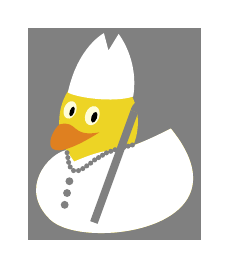
\begin{tikzpicture}
\fill[gray] (0,0) rectangle (2.2,2.7);
	\duck[tshirt=white,necklace=gray,buttons=gray,crozier=gray]
	\path[fill=white] (0.5101,1.8761) .. controls (0.6355,2.4588) and (0.9681,2.6303) .. (0.9681,2.6303) -- (1.0260,2.4101) -- (1.1548,2.6202) .. controls (1.1548,2.6202) and (1.4167,2.2951) .. (1.3398,1.8247) .. controls (1.0829,1.7440) and (0.6286,1.8104) .. (0.5101,1.8761) -- cycle;
\end{tikzpicture}	
	
\end{document}